

In diesem Kapitel wird die Theorie aus dem Kapitel Analyse in ein funktionsfähiges VHDL-Programm mit den geforderten Eigenschaften
umgesetzt.
Es werden weitere Vorüberlegungen getroffen, die sich speziell an der Implementation als Hardwarekomponente orientieren.
Wenn die Komponente Teil eines Chips werden würde, wurde dieser in $\SI{350}{nm}$ Technologie gefertigt werden. Entprechend beziehen
sich die Größenangaben der Syntheseergebnisse auf diesen Prozess. Der Auftragsfertiger, bei dem der Chip in Auftrag gegeben werden würde, ist
Austria Micro Systems (AMS). Dementsprechend sind die Standarzellen von dieser Firma.


\section{Projekt- und Programmstruktur}
In diesem Abschnitt werden Entscheidungen zum Einhalten der Bitbreite der Vektoren, den verwendeten VHDL-Bibliotheken und der Aufteilung des Programmcodes zusammengetragen.

 \subsection{Vorüberlegungen aus Hardwaresicht}
 Für die binäre Darstellung der Eingangswerte sind zwölf Bit vorgesehen, wovon zehn auf die 
 Nachkommastellen entfallen. Bei den beiden Rechenoperationen Addition und Subtraktion
 entstehen keine weiteren Nachkommastellen. Je nach Vorzeichen und Zahlenwert kann es jedoch sein,
 dass der Vorkomma-Wertebereich von zwei Bit nicht mehr ausreicht. Aus diesem Grund muss der Zielvektor
  immer um ein Bit breiter sein - von 12 Bit ausgehend also 13 Bit.
  Da dies bei jeder Addition geschieht, würde die benötigte Bitbreite ohne Gegenmaßnahmen immer 
  weiter anwachsen. Die einfachste Möglichkeit dies zu verhindern ist die Divison eines Summationsergebnises
  durch Zwei. 
  So kann beliebig oft auf den selben Vektor eine Addition ausgeführt werden, ohne einen Überlauf zu provozieren.
  Die Kehrseite dieser Vorgehensweise ist, dass durch den Bitshift die Genauigkeit des Ergebnisses sinkt.
  Auf die Folgen wird in Abschnitt \ref{sec:NumerischeUngenauigkeiten} kurz eingegangen.
  Für die verlustfreie Multiplikation zweier Zahlen wird sogar die doppelte Breite des Vektors 
  benötigt. Hier kann sich der Bitbereich vor und nach dem Komma ändern.
  
  Wenn diese Maßnahme jedoch nicht ergriffen und alle zusätzlichen Bits beibehalten 
  würden, müsste mit etwa 70 Bit je Ausgangswert gerechnet werden. Sollte wenigstens
  auf die bei der Multiplikation entstehenden Nachkommabits verzichtet werden, 
  würde die benötigte Bitbreite immer noch bei über 40 liegen.
  Auch dies würde noch eine immense Vergrößerung der Schaltung alleine schon wegen der zusätzlichen
  Leitungen bedeuten. Desweiteren würden sich hierdurch die benötigten Zeiten aller Berechnungen erhöhen, 
  was eine langsamere Taktfrequenz oder eine eine Unterteilung in Teilschaltnetzte und somit in der Summe
  mehr Takte mit sich ziehen würde.
  




 
 
 \subsection{VHDL-Bibliotheken}
 Cadence unterstützt die VHDL-Versionen von 1987 und 1993. 
 Enthalten ist unter anderem die Bibliothek \texttt{std\_logic\_arith}, welche von der Firma Synopsys entwickelt wurde. Hierbei handelt es sich um die erste Bibliothek
 für mathematische Berechnungen wie Addition und Multiplikation mit VHDL, weshalb sie eine große Verbreitung erlangt hat.
 Die Bibliothek basiert auf der vom Konsortium des Institute of Electrical and Electronics Engineers (IEEE) spezifizierten Bibliothek \texttt{std\_logic}. Anders als angenommen werden könnte, handelt es sich hierbei nicht um einen offiziellen Standard.
 Ähnliches gilt auch für die Bibliotheken \texttt{std\_logic\_unsigned} und \texttt{std\_logic\_signed}.
 Leider hat Synopsys nicht konsequent die strenge Typisierung von VHDL eingehalten, weshalb es bei überladenen Funktionen möglich ist, die Datentypen \texttt{signed} und \texttt{unsigned} zu mischen, was zu einem unerwarteten Verhalten führt.
 Aus diesem Grund wird in diesem Projekt die Bibliothek \texttt{numeric\_std} verwendet, welche einen vergleichbaren Funktionsumfang bietet, vom IEEE-Konsortium spezifiziert wurde und dieses Problem nicht aufweist. Zu ihrem 
 Umfang gehört auch die \texttt{resize}-Funktion, welche es ermöglicht einen Vektor vorzeichengerecht zu erweitern.
 
Für den Standardsatz der Datentypen zu dem beispielsweise \texttt{std\_logic} gehört, wird 
\texttt{std\_logic\_1164.all} verwendet.
Um Textdateien lesen und schreiben zu können, wird die Bibliothek \texttt{std.textio.all} sowie 
\texttt{std\_logic\_textio.all} benötigt.

%Die im Jahr 2008 veröffentlichte VHDL-Version führt Unterstütztung mit den Datentypen \texttt{ufixed} und 
%\texttt{sfixed} die Möglichekeit ein, (vorzeichenbehaftete) Kommazahlen zu verwenden. Die 
 
\subsection{Vorüberlegungen zum Programmablauf}\label{sec:VorueberlegungenProgrammablauf}
Über die Parallelität der Berechnungen wird auch bei gleicher Funktion der Komponenten maßgeblich die benötigten Takte der Berechnung der 2D-DFT sowie die benötigte
Logik und deren Größe bestimmt. 
% Für die Aufwandsabschätzung wird angenommen, dass alle Eingangswerte zeitgleich zur Verfügung stehen.
Um einen guten Kompromiss aus benötigter Zeit und Chipfläche zu erzielen,
sollen  Real- und Imaginärteil die die Berechnung der Matrixelemente jeweils gleichzeitig, die einzelnen Elemente aber nacheinander berechnet werden. Darüber hinaus ist geplant, die selbe Recheneinheit der 1D-DFT auch für die 2D-DFT zu nutzen. 


\subsection{Struktureller Aufbau}
 Das Programm wurde, wie bei umfangreicheren Projekten üblich, auf verschiedene Dateien aufgeteilt. Alle Konstanten werden in einem Paket deklariert, welches in allen anderen Dateien
 eingebunden werden muss. So ist es möglich z.B. die Bitbreiten eines Vektors an einer zentralen Stelle zu setzen. Diese liegen für 
 Eingangswerte bei 12, Summen 13 und Produkte 26 Bit. Da alle anderen Dateien auf diese
 Konstanten zugreifen, muss dieses Paket zuerst kompiliert werden. In einem weiteren Paket findet die Deklaration der eigenen Datentypen statt. Hier sei
 insbesondere die 8x8 Matrix mit ihren 12 Bit Vektoren vom Typ \texttt{signed} erwähnt, welche für die eingelesenen 
 Daten, die Zwischenergebnisse (1D-DFT) sowie die Ausgangswerte verwendet wird.
 Da die weiteren Dateien diese Datentypen verwenden, ist es 
 erforderlich, dass dieses Paket als zweites kompiliert wird. Alle weiteren Pakete können in beliebiger Reihenfolge kompiliert werden, da sie erst später ineinander
 greifen. 
 Zum Testen bzw. für die Simulation müssen Eingangswerte geladen werden. Hierfür wurde die Komponente \texttt{read\_input\_matrix} geschrieben. Die Werte müssen
 in einer Datei mit dem Namen \texttt{InputMatrix\_komplex.txt} stehen und im dualen Zahlenformat vorliegen. 
 Die Datei besteht aus 16 Spalten und acht Zeilen, in den leerzeichengetrennten Spalten stehen immer im Wechsel der Real- und der Imaginärteil einer Zahl.
  Die berechneten Ergebnisse werden mit der Komponente \texttt{write\_results} im gleichen Format in eine Datei geschrieben, wie sie in der Input-Datei stehen. 



\section{Entwicklung der 2D-DFT-Komponente}
Bis die Berechnung der 2D-DFT realisiert war, wurden verschiedene Stadien durchlaufen. Im ersten Schritt wurde die 1D-DFT implementiert, wobei die im Kapitel
Analyse behandelten Optimierungsmöglichkeiten näher betrachtet werden. Desweiteren wird das Berechnungsschema der geraden sowie ungeraden Zeilen der 
Twiddlefaktormatrix und die daraus resultierende Anzahl an Takten vorgestellt.
Ein weiterer wichtiger Punkt ist die Umsetzung der 2D-DFT auf Basis der vorhandenen 1D-DFT-Einheit.
Abschließend wird gezeigt, dass es auf einfache Weise möglich ist, die vorhandene DFT-Einheit um die Funktion der IDFT zu ergänzen.




\subsection{Optimierte 8x8 DFT als Matrixmultiplikation}\label{sec:OptimierteMatrixmultiplikation}
Anfangs wurde angenommen, dass Multiplikationen mit den Twiddlefaktoren $\pm 1$ und $\pm\frac{\sqrt{2}}{2}$ durchgeführt werden müssen. 
Dass bei einer optimierten 8x8-DFT wegen des explizieten ausprogrammierens der Berechnungen die Multiplikation mit $\pm1$ wegfällt, war schnell klar.
Wegen der betragsmäßig identischen nicht trivialen Twiddlefaktoren wurde zu Beginn der Entwicklung in Betracht gezogen das 1er-Komplement zu verwenden, da sich negative und positive Zahlen mit gleichem Betrag nur durch ihr höchstwertigstes 
Bit unterscheiden. Auf diese Weise könnte dasselbe Resultat für den Imaginär- wie für den Realteil verwendet werden. Das Vorzeichen würde sich über eine 
einfache XOR-Verknüpfung beider MSB der Multiplikanden ergeben.
Diesem Vorteil steht jedoch eine aufwändigere Subtraktion (bzw. Addition negativer Zahlen) gegenüber. Der zusätzliche Aufwand entspricht 
etwa dem der Negierung von Zahlen im 2er-Komplement. Aus diesem Grund wurde sich hierfür entschieden.

Bei der genaueren Betrachtung der Twiddlefaktormatrix konnte in Abschnitt \ref{sec:KomplexeEingangswerte} festgestellt werden, dass, abgesehen von der ersten, in jeder Zeile gleich viele Additionen wie Subtraktionen vorhanden sind. Dies trifft auch ausschließlich auf die jeweils vier nicht trivialen Faktoren der geraden Zeilen zu. 
Dies lässt sich anhand des Einheitskreises in Abb. \ref{pic:Einheitskreis_Faktoren}, der Abbildung \ref{pic:Twiddlefaktoren_Darstellung8x8}
 und der grafischen Darstellung der Twiddlefaktormatrix in Abb. \ref{pic:MatrizenDarstellungTwiddlefaktoren} nachvollziehen. 
% In der letztgenannten ist zu sehen, dass die 2., 4., 6., und 8. Zeile je vier nicht triviale und komplexe Faktoren enthält. 
 Darüber hinaus ist ersichtlich, dass für komplexe Eingangswerte in den Zeilen 2, 4, 6 und 8 zwölf und in den übrigen acht Multiplikationen erfolgen müssen. Dies kann anhand der 
 Gleichungen (\ref{eq:komplexe_Multiplikation}) und (\ref{eq:halb_komplexe_Multiplikation}) nachvollzogen werden.
 %Das lässt sich ausnutzen, um keine Negationen der Eingangs- und Zwischenwerte durchführen zu müssen. 
 
Aus Abschnitt \ref{sec:Matrixmultiplikation} ist bekannt, dass bei einer Matrixmultiplikation Elemente multipliziert und anschließend die Ergebnisse 
 aufsummiert werden.
 Hieraus kann abgeleitet werden, dass es das Assoziativgesetz erlaubt die Eingangswerte umzusortieren, wenn auch die Twiddlefaktoren entsprechend umsortiert werden. 
Geschickt aufgeteilt auf triviale und nicht triviale Berechnungen, 
ist es dadurch möglich auf das Invertieren der Eingangswerte, also den hierfür benötigten Takt und die Inverter zu verzichten und um nur noch die Multiplikation
mit $+\frac{\sqrt{2}}{2}$ durchführen zu müssen. Letztere muss wegen des Distributivgesetzes nur ein Mal pro Zeile und Real- bzw. Imaginärteil erfolgen.

 Darüber hinaus minimiert sich bei dieser Anordnung das Risiko eines Überlaufs, da zumindest im ersten Schritt eine Subtraktion erfolgt. In den weiteren muss unweigerlich die 
 Akkumulation stattfinden. 
 Wegen der Einsen in der ersten Zeile der Twiddlefaktormatrix müssen für die erste Zeile der Ausgangsmatrix alle Spalten einmal aufsummiert werden.
 Dies hat zur Folge, dass ein großer Wert entstehen kann, welcher Maßgebend für die Anzahl der Vorkommabits ist.
 Aus diesem Grund wird zur Sicherheit, der einheitlichen Skalierung der Zahlen und der Einfachheit wegen nach jeder Addition oder Subtraktion das Ergebnis durch einen Bitshift halbiert. 
 Es sei an dieser Stelle lediglich angemerkt, dass über die Eingangswerte die Annahme getroffen werden kann, dass aufeinanderfolgende Werte das selbe Vorzeichen haben oder, nach Abzug eines evtl. vorhandenen Offsets, nahe Null sind. 
 Basierend auf diesem Wissen ist es denkbar die Wahrscheinlichkeit weiter zu reduzieren, dass es zu einem Überlauf kommt. 
Wegen der Null im Imaginärteil der ersten und fünften Zeile der Twiddlefaktormatrix sind auch alle Imaginärteile dieser Spalte der Ausgangsmatrix Null.
Wie in Abschnitt \ref{sec:NumerischeUngenauigkeiten} erwähnt, ist die Optimierung bezüglich numerischer Ungenauigkeiten nicht Gegenstand dieser Arbeit.

 
 
\subsection{Berechnungsschema und benötigte Takte der Ergebnisse}\label{sec:Berechnungsschema}

In Abbildung \ref{pic:AkkumulationUngeradeSpalten} ist die Berechnung der ungeraden Spalten der Eingangsmatrix am Beispiel der ersten zu sehen. Für die 3. und 7. müssen die 
Eingangswerte so angeordnet werden, dass die Vorzeichen, beginnend mit einer Subtraktion, immer im Wechsel auftreten. Für die 5. Zeile ist dies bereits gegeben.
$r$ steht für den Realteil der Eingangswerte, $i$ stünde für dessen Imaginärteil. Der Index gibt die Postition des Elements in einer Spalte an, angewandt werden muss die
Berechnung auf alle Spalten.


\begin{figure}[htbp]
\centering
1. Spalte:\quad $r_{0} + r_{1} + r_{2} + r_{3} + r_{4} + r_{5} + r_{6} + r_{7}$\\

\vspace{0.5cm}
\begin{tabular}{ccccccccc}
Takt&\multicolumn{6}{l}{ } & & Bit\\
1&$\underbrace{r_{0} + r_{1}}$ &  &$ \underbrace{r_{2} + r_{3}}$ &  &$\underbrace{r_{4} + r_{5}}$ &  &$\underbrace{r_{6} + r_{7}}$ & 12\\
&\multicolumn{7}{l}{$\hspace{0.65cm} \Downarrow \hspace{2.3cm} \Downarrow \hspace{2.3cm} \Downarrow \hspace{2.3cm}\Downarrow$}&13\\
2&\multicolumn{3}{c}{$\underbrace{sum\_1\_1 \quad + \quad sum\_1\_2}$} & & \multicolumn{3}{c}{$\underbrace{sum\_1\_3 \quad + \quad sum\_1\_4}$} & 12\\
&\multicolumn{3}{c}{$\Downarrow$} & & \multicolumn{3}{c}{$\Downarrow$}&13\\
3&\multicolumn{7}{c}{$\underbrace{sum\_2\_1 \quad  \quad \quad \quad + \quad \quad \quad  \quad sum\_2\_2}$} & 12\\
&\multicolumn{7}{c}{$\Downarrow$}&13\\
&\multicolumn{7}{c}{$sum\_3\_1$} & 12\\
&\end{tabular}
%\captionof{figure}{Vorgehensweise der Akkumulation der ungeraden Spalten der Eingangswerte}
\caption{Vorgehensweise der Akkumulation der ungeraden Spalten der Eingangswerte.}
\label{pic:AkkumulationUngeradeSpalten}
\end{figure}
%\end{center}

Wie der linken Spalte der Abb. \ref{pic:AkkumulationUngeradeSpalten} zu entnehmen ist, werden 3 Takte für die Berechnungen der Werte aus den ungeraden Spalten der Eingangsmatrix benötigt.
Der 1. Takt für Additionen bzw. Subtraktionen und 2. sowie 3. Takt für das Aufsummieren. Der Bitvektor des Ergebnisses ist zwar 12 Bit breit, aber beim letzten Bitshift von 13 auf 12
werden nur 11 Bit übernommen. Es wird alo ein doppelter Bitshift vollzogen. Dies erfolgt, damit sowohl in den geraden als auch den ungeraden Zeilen gleich viele Bitshifts erfolgen
und die Werte somit identisch skaliert sind.

Die Berechnung der geraden Zeilen wird in Abbildung \ref{pic:AkkumulationGeradeSpalten} am Beispiel der zweiten Zeile gezeigt.
$r$ steht wieder für den Realteil der Eingangswerte, $i$ für dessen Imaginärteil. 
Auch hier ist der linken Spalte die Anzahl der benötigten Takte zu entnehmen. In diesem Fall dauert die Berechnung 5 Takte. Diese setzen sich zusammen aus
ein Takt für Additionen bzw. Subtraktionen, 2.-3. sowie 5. Takt für das Aufsummieren und der 4. Takt für die Multiplikationen.
In Abschnitt \ref{sec:Konstantenmultiplizierer} wird gezeigt, dass die Multiplikation mit einer Konstanten innerhalb eines Taktes mit einem Schaltnetz erfolgen kann. 

\begin{figure}[htbp]
 \centering
 
2. Spalte:  $r_1 - r_3 + i_1 - i_7 + i_3 - r_5 + r_7 - i_5 + r_0 - r_4 + i_2 - i_6$
 
 %$a_0 - x_1 + x_0 - b_2 + x_2 - x_3 + a_4 - x_5 + x_4 - b_6 + x_6 - x_7$\\

 \vspace{0.3cm}
 
\begin{tabular}{ccccccccccccc}
Takt&\multicolumn{11}{c}{}&Bit\\
1 &$\underbrace{r_1 - r_3}$ &        &$ \underbrace{i_1 - i_7}$ &  &$\underbrace{i_3 - r_5}$ &  &$\underbrace{r_7 - i_5}$ &  &$\underbrace{r_0 - r_4}$ &$\underbrace{i_2 - i_6}$& &12\\
  &\multicolumn{11}{l}{$\hspace{0.5cm} \Downarrow \hspace{1.75cm} \Downarrow \hspace{2.4cm} \Downarrow \hspace{1.8cm}\Downarrow \hspace{1.8cm}\Downarrow \hspace{1.4cm}\Downarrow$}&13\\
2 &\multicolumn{3}{c}{$\underbrace{sum1\_1 \: + \: sum1\_2}$} & & \multicolumn{3}{c}{$\underbrace{sum1\_3 \: + \: sum1\_4}$} &\multicolumn{3}{c}{$\: \underbrace{sum1\_5 \: + \: sum1\_6}$}& &12\\
  &\multicolumn{3}{c}{$\Downarrow$}  & & \multicolumn{3}{c}{$\Downarrow$} & & \multicolumn{2}{c}{$\Downarrow$}& &13\\
3 &\multicolumn{7}{c}{$\underbrace{sum2\_1 \quad  \quad \quad \quad + \quad \quad \quad  \quad sum2\_2}$} & & & & &12\\
  &\multicolumn{7}{c}{$\Downarrow$}& & \multicolumn{2}{c}{$\Downarrow$}& &13\\
  &\multicolumn{7}{c}{$sum3\_1$}& & & & &13\\
  & & & & $\Downarrow$& & & & & \multicolumn{2}{c}{$\Downarrow$} & & 13\\
4 & & & & $\frac{\sqrt{2}}{2}$&\multicolumn{5}{c}{}& & &13\\
  & & & & $\Downarrow$& & & & & \multicolumn{2}{c}{$\Downarrow$ }& & 26\\
5 & & & \multicolumn{9}{c}{$\underbrace{sum4\_1 \:  \quad \quad \quad \quad \quad \quad + \quad \quad \quad \quad \quad \quad   sum2\_3}$} &12\\
  & & & \multicolumn{9}{c}{$\Downarrow$}&13\\
  & & & \multicolumn{9}{c}{$sum5\_1$}&12\\
\end{tabular}
\caption{Vorgehensweise der Akkumulation und Multiplikation der geraden Spalten der Eingangswerte.}
\label{pic:AkkumulationGeradeSpalten}
\end{figure}



Der rechten Spalte aus Abb. \ref{pic:AkkumulationGeradeSpalten} kann entnommen werden, dass sich durch die Addition eine Bitbreitenerweiterung um eins bzw. bei der Multiplikation eine Verdoppelung ergibt. 
% Bei einer früheren 
% Implementierung, die nur die 1D-DFT beherrschte, wurde zumindest die Erweiterung bei der Addition umgesetzt. Da bei der 2D-DFT die selbe Recheneinheit genutzt 
% werden soll, wurde in Absprache mit dem ISAR-Team entschieden, dass die Summanden vor jeder Summation durch einen Bitshift nach rechts halbiert werden. Auf diese
% Weise hat ein Additionsergebnis immer 13 Bit Breite. Durch den Bitshift kann das Resultat der 1D-DFT direkt als Eingang für die 2D-DFT verwendet werden. 
Durch die hintereinander erfolgenden Bitshifts wird durch $2^{n_B}$ geteilt, 
wobei $n_B$ die Anzahl der Bitshifts ist. Den beiden Darstellungen der Summationen kann entnommen werden, dass, um ein Überlaufen des Bitvektors zu vermeiden es nötig ist,
drei respektive vier Bitshifts durch zu führen. Wie bereits erläutert erfolgt bei den ungeraden Zeilen abschließend ein doppelter Bitshift. Auf diese Weise ergibt sich für die
1D-DFT, dass das Ergebnis um den Faktor 16 kleiner ist. Da beim zweiten Durchlauf, um die 2D-DFT zu berechnen, ebenfalls 
durch 16 geteilt wird, ergibt sich insgesamt eine Division durch $2^{2\cdot4} = $ 256.

Aus den Abbildungen \ref{pic:AkkumulationUngeradeSpalten} und \ref{pic:AkkumulationGeradeSpalten} können die Takte, die zur Berechnung der 1D- bzw. 2D-DFT benötigt werden, 
abgeleitet werden.
Für ungeraden Zeilen sind je Element drei Takte nötig und mit acht Elementen pro Zeile und vier ungeraden Zeilen errechnen sich so 3$\cdot$8$\cdot$4=96 Takte.
Analog errechnet sich für die geraden Zeilen mit je fünf Takten pro Element 5$\cdot$8$\cdot$4=160 Takte.
In der Summe ergeben sich so 96+160=256 Takte für die 1D-DFT. Da die 2D-DFT ohne Takte fürs Umspeichern oder ähnliches sofort im Anschluss berechnet werden kann, 
verdoppelt sich die Anzahl der Takte auf 512 für die vollständige Berechnung.

\begin{table}[ht!]
\centering
\caption{Benötigte Takte für die komplexe DFT}
\label{tab:TakteKomplexeDFT}
\begin{tabular}{ccccc}
\hline
\multirow{2}{*}{Zeile} & Additionen & Takte pro Element & Takte für & Summe der\\
      & pro Element ($N$) & ($\log_2(N)$) & Multiplikation & Takte\\
\hline
 1& 8  & 3   &0 &3\\
 2& 12 & 3,6 &1 &5\\
 3& 8  & 3   &0 &3\\
 4& 12 & 3,6 &1 &5\\
 5& 8  & 3   &0 &3\\
 6& 12 & 3,6 &1 &5\\
 7& 8  & 3   &0 &3\\
 8& 12 & 3,6 &1 &5\\
\hline
\end{tabular}
\end{table}

Anhand der rechten Spalte ergeben sich so (3+5)$\cdot$4$\cdot$8 = 256 Takte sowohl für den Real- als auch den Imaginärteil der komplexen Ausgangsmatrix. Real- und Imaginärteil
werden parallel berechnet und sind somit zeitgleich fertig.


\subsection{Programmablauf der 1D-DFT}\label{sec:Programmablauf1D}
Im ersten Takt der Berechnung werden die für die jeweilige Zeile der Twiddlefaktormatrix spezifischen Additionen und Subtraktionen durchgeführt. 
Für die geraden Zeilen werden die Werte, die eine Multiplikation benötigen, getrennt von den übrigen zusammengefasst.
Im darauffolgenden Takt werden die Zwischenwerte, für die geraden Zeilen wieder getrennt nach Multiplikation oder nicht, akkumuliert.
Der dritte Takt ist für die ungeraden Zeilen der letzte, da nur acht Werte aufsummiert werden müssen (siehe Abb. \ref{pic:AkkumulationUngeradeSpalten}). 
Im darauffolgenden Takt wird in den ungeraden Zeilen mit der Berechnung der nächsten Zahl begonnen.
Die geraden Zeilen haben acht Werte, die mit $\nicefrac{\sqrt{2}}{2}$ multipliziert werden müssen. Die vier Werte, die nur addiert werden müssen, sind bereits im zweiten Takt 
aufsummiert. Deshalb kann im vierten Takt die Konstantenmultiplikation erfolgen und abschließend im fünften die Summation der Zwischenergebnisse erfolgen (siehe Abb. \ref{pic:AkkumulationGeradeSpalten}).

Die Zuordnung der aktuellen Zeile der Twiddlefaktormatrix erfolgt über einen Zähler, der von 0 bis 63 zählt. Er ist als 6 Bit Vektor realisiert, der bei 63 einen beabsichtigten Überlauf hat und wieder bei 0 anfängt.
Der Vektor kann als zwei aufeinanderfolgende 3 Bit Vektoren gesehen werden. Auf den vorderen wird immer eine Eins aufaddiert, wenn der hintere einen Überlauf hat und wieder bei Null zu zählen beginnt. Beide Vektoren können für sich als Modulo-8-Zähler betrachtet werden.
Die vorderen drei Bit des gesamten Vektors entsprechen der aktuellen Zeile, die hinteren drei der Spalte, also dem Index in der aktuellen Zeile.
Mit der Funktion \texttt{to\_integer} der VHDL-Bibliothek \texttt{numeric\_std} lassen sich die Teilvektoren nutzen, um die Elemente der Eingangsmatrix anzusprechen.
Das letzte Bit des ersten Teilvektors ist für ungerade Zeilen Null und für gerade Zeilen Eins.
Da sich die Eigenschaften der Twiddlefaktormatrix in gerade und ungerade Zeilen aufteilen lassen, kann dies genutzt werden, um die entsprechenden Operationen durchzuführen und den passenden Folgezustand des Zustandsautomaten zu setzen.


\subsection{Entwickelung von der 1D-DFT zur 2D-DFT}
In Abschnitt \ref{sec:VorueberlegungenProgrammablauf} wurde entschieden, dass nach Möglichkeit die selbe Recheneinheit
für die 1D- wie auch die 2D-DFT genutzt werden soll. 
Aus Abschnitt \ref{sec:2d-dft} ist bekannt, dass für die 2D-DFT einer Matrix die Twiddlefaktormatrix einmal links und einmal rechts von der Eingangsmatrix steht.
Als 1D-DFT-Matrix (Zwischenwertematrix) wird die Multiplikation der ersten Twiddlefaktormatrix mit der Eingangsmatrix betrachtet. Anschließend wird die 1D-DFT-Matrix mit der 
Twiddlefaktormatrix multipliziert. Aus der vertauschten Reihenfolge resultiert, dass die Zeilen und Spalten getauscht durchlaufen werden. 
Da die Eingangsmatrix spaltenweise durchlaufen werden soll, müsste  für jedes Element eine aus Hardwaresicht aufwändige Fallunterscheidung erfolgen.
Umgehen lässt sich dass, indem das Kommutativgesetz angewandt wird und die Matrizen transponiert werden. Belegt wird das mit der Gleichung (\ref{eq:MatMultTranspose}). Wie zu sehen ist, muss auch die Ausgangsmatrix transponiert werden. Für die Twiddlefaktormatrix erübrigt sich dies, da ihre Transponierte identisch ist.
Es konnte gezeigt werden, dass beide Berechnungen mit der selben Einheit durchführbar sind. In Grafik (\ref{pic:MatMultTranspose}) ist das beschriebene veranschaulicht.
Das Transponieren der Zwischen- und der Ausgangsmatrix erfolgt mit vertauschtem Zeilen- und Spaltenindex. 
Für die Unterscheidung zwischen 1D- und 2D-DFT wird ein Bit-Signal getoggelt, wenn der in Abscnitt \ref{sec:Programmablauf1D} eingeführte Vektor bis 63 gezählt hat.

\begin{align}
 X &= W \cdot x \cdot W \nonumber \\
   &= \left(\left(x\cdot W\right)^T\cdot W\right)^T \label{eq:MatMultTranspose}\\
   &= \left(X^{*T} \cdot W\right)^T \nonumber
\end{align}


\begin{figure}[htbp]
 \centering
 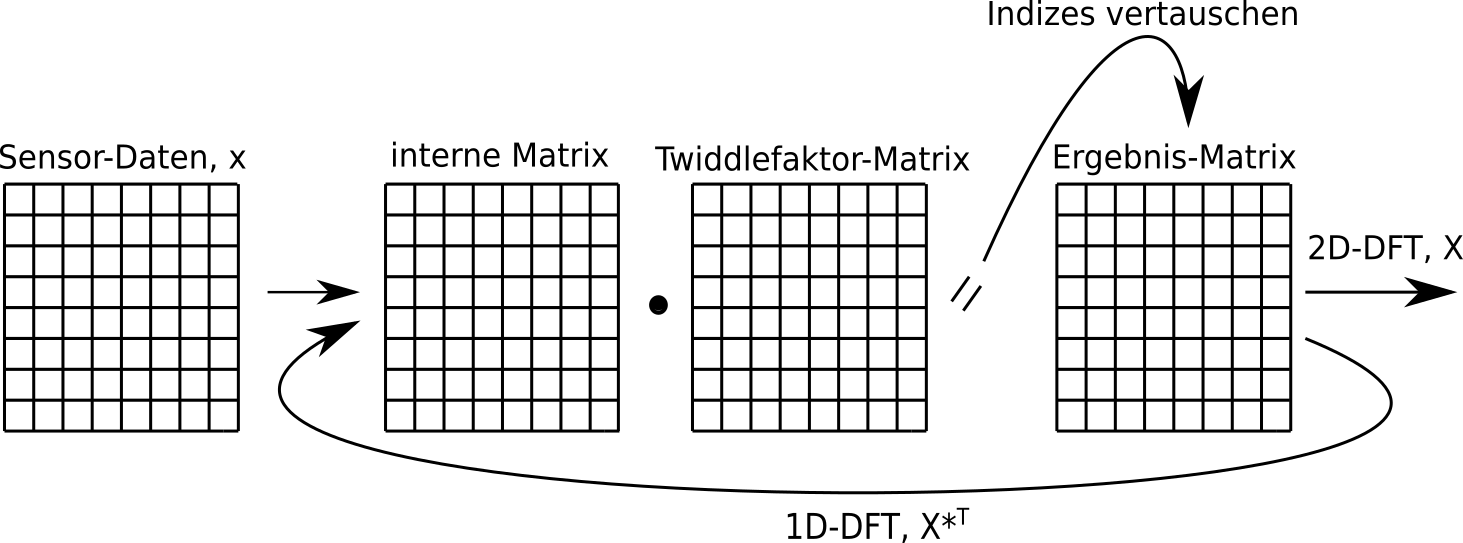
\includegraphics[width=0.95\textwidth]{img/MatMultTranspose2.png}
 \caption{Darstellung der Berechnung der 2D-DFT aus Gleichung (\ref{eq:MatMultTranspose}).}
 \label{pic:MatMultTranspose}
\end{figure}




Da die Matrizen transponiert werden, ist eine zweite interne Matrix erforderlich, da sonst die Werte oberhalb der
Nebendiagonalen überschrieben werden.

% 
% \subsection{Direkte Weiterverarbeitung der Zwischenergebnisse}
% Um die Anzahl an Gattern und somit den Flächenbedarf zu reduzieren ist es das Ziel, die Ergebnisse der \gls{1d-dft} aus der 1. Berechnungsstufe im nächsten Schritt direkt als 
% Eingangswerte für die \gls{2d-dft} zu verwenden. Auf diese Weise würden 64$\cdot$2$\cdot$12 Bit = 1536 Bit = 1,5kBit = 192 Byte an Speicher eingespart werden.
% Wie sich im Laufe der Entwicklung gezeigt hat, lässt sich das nicht nutzen. Das liegt daran, dass dazu übergegangen wurde, immer nur ein Element zur Zeit berechnet wird und die 
% bereits errechneten demnach zwischengespeichert werden müssen. Dieser Ansatz wurde verfolgt, da der Entwicklungsaufwand in VHDL für die spaltenweise Berechnung der Ausgangswerte 
% einfacher umzusetzen war und es zunächst nur um die mathematische Umsetzung und nicht um die Platzeffizienz auf einem Chip ging.
% 
% Unklar war zu diesem Zeitpunkt noch, wie der Speicher realisiert werden soll. In der finalen Variante des Chips soll es einen \gls{ram} geben, der als zentraler
% Speicher von allen Komponenten genutzt wird. Da die Entwicklung im Projekt noch nicht soweit fortgeschritten ist und dies nicht zu den Aufgaben der vorliegenden Arbeit gehört,
% wurde auf das Speichern in lokalen Speicherzellen ausgewichen, welche als Variable oder Signal im VHDL-Code definiert und von der Software als Flip-Flop synthetisiert werden.
% 
% 


\subsection{Zusammenhang von DFT und IDFT bei der Matrixmultiplikation}\label{sec:idft}

Durch die umgekehrte Drehrichtung des komplexen Zeigers in Gleichung (\ref{eq:idft}) werden in der Matrizenschreibweise die Zeilen 2 und 8, 3 und 7 sowie 4 und 6 vertauscht.
Nachvollziehen lässt sich das gut anhand der Grafik \ref{pic:Einheitskreis_Faktoren}. 
Verdeutlicht wird das vorgehen in Abbildung \ref{pic:IDFT_Zeilentausch}.

Dies lässt sich nutzen, um auf einfache Weise die vorhandene DFT-Einheit um die IDFT-Funktionalität zu ergänzen. 
Die DFT-Komponente wird dafür um das Eingangssignal \texttt{idft} ergänzt. Im Quelltext erfolgt eine Abfrage, ob \texttt{idft} gesetzt ist. Ist dies der Fall, wird der 
in Abschnitt \ref{sec:Programmablauf1D} eingeführten Teilvektor für das Durchlaufen der Zeilen in seiner Integer-Interpretation von Acht subtrahiert.

\begin{figure}[ht]
 \centering
 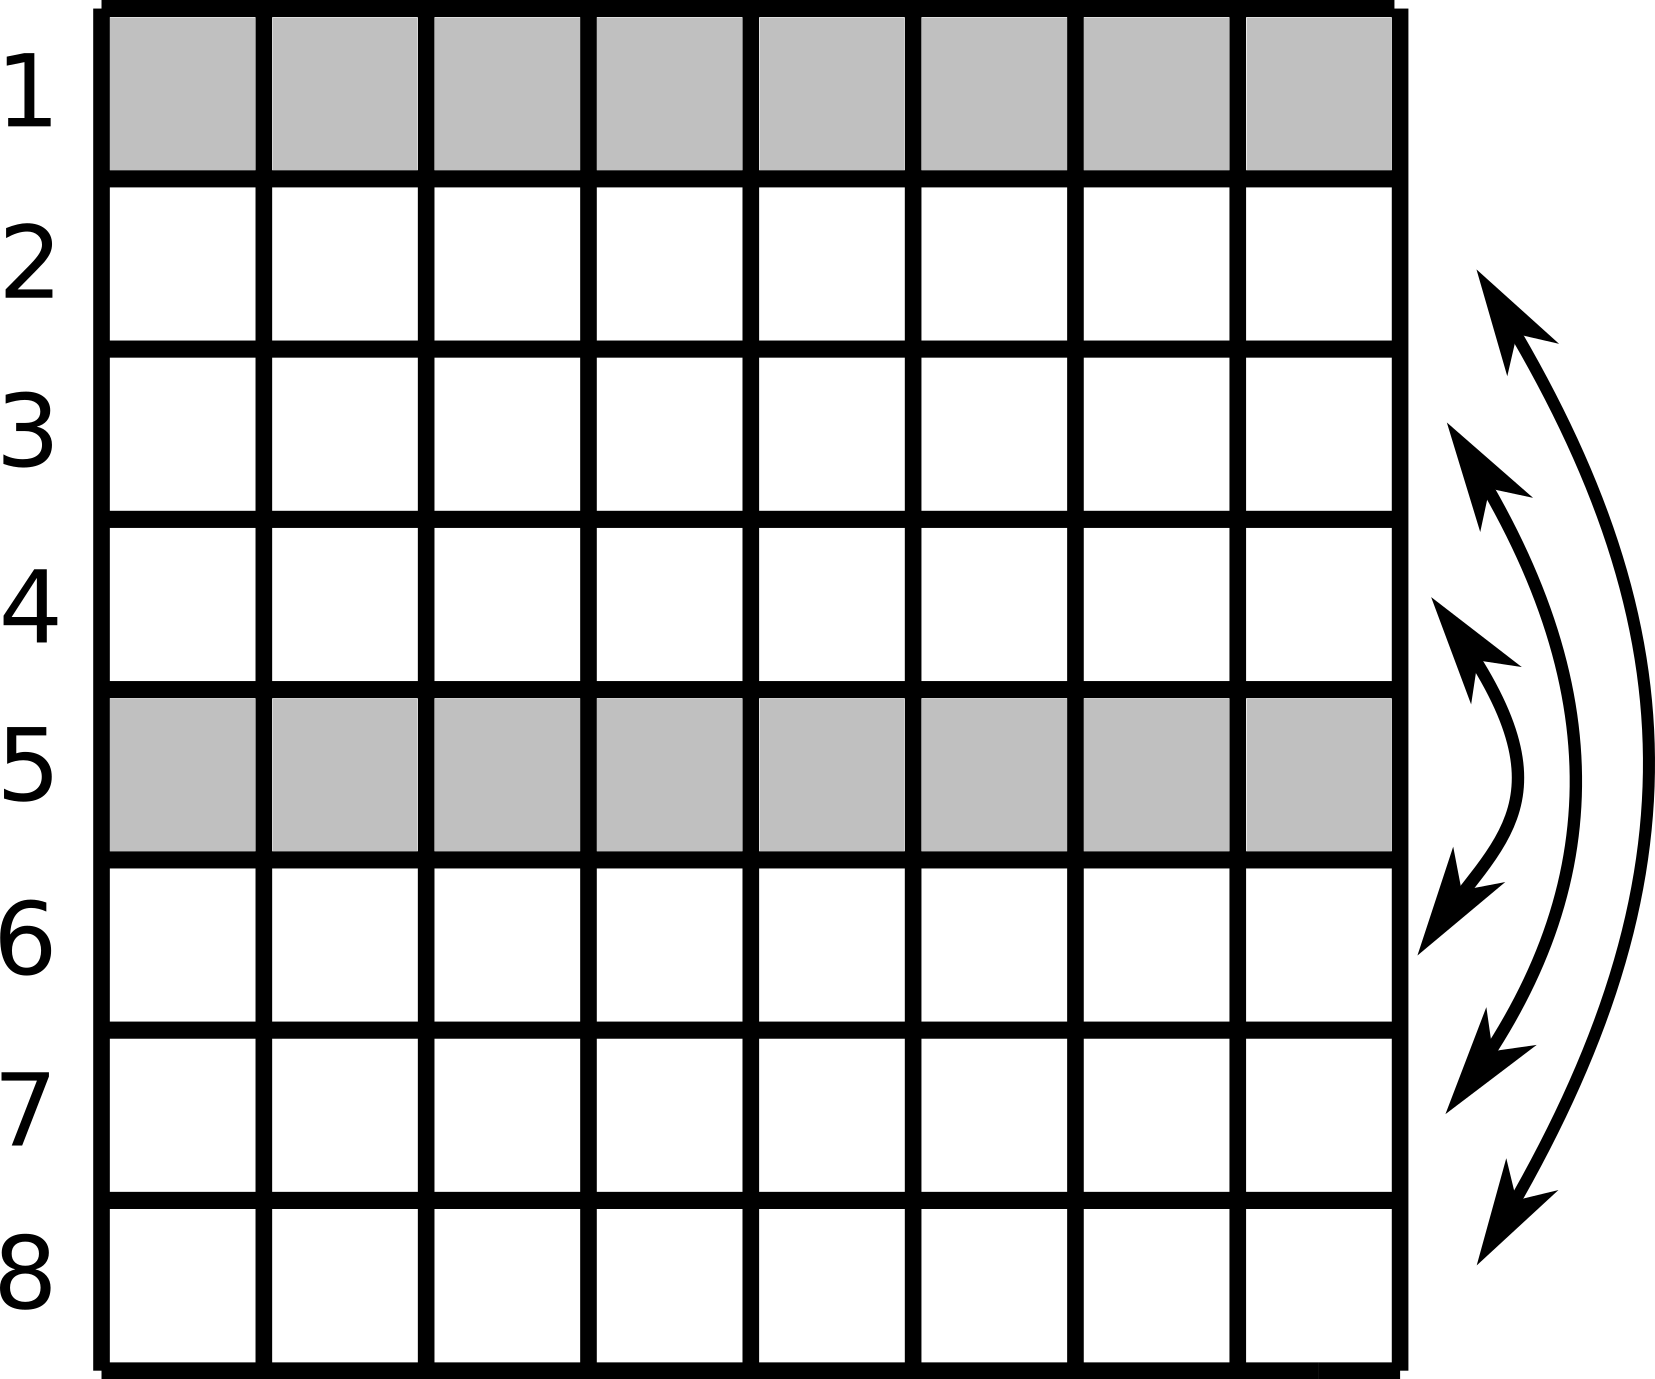
\includegraphics[width=0.4\textwidth]{img/IDFT_Zeilentausch.png}
 \caption{Vertauschen der Zeilen 2 und 8, 3 und 7 sowie 4 und 6 der Twiddlefaktormatrix, um von der DFT zur IDFT zu gelangen.}
 \label{pic:IDFT_Zeilentausch}
\end{figure}




\section{Syntheseergebnisse von Teilkomponenten}\label{sec:Syntheseergebnisse}
Die Syntheseergebnisse werden mit dem Programm \texttt{rc} erstellt. Wenn 
Da das Schaltnetz der gesamten Schaltung zu groß und nicht nachvollziebar wäre, werden in diesem Abschnitt nur relevante Teilkomponenten gezeigt.

\subsection{13 Bit Konstantenmultiplizierer}\label{sec:Konstantenmultiplizierer}

Der duale Wert lässt sich am einfachsten mit der Matlab-Funktion \texttt{fi()} ermitteln. Der Funktion werden hierfür Kommagetrennt der Deziamlwert, 1 für vorzeichenbehaftet,
die gesamte Anzahl an Stellen (13) und die Anzahl der Nachkommastellen (10) übergeben. Der vollständige Aufruf sieht dann wie folgt aus:

\texttt{val=fi(sqrt(2)/2,1,13,10)}

Der erzeugte Datentyp hat unter anderem die Eigenschaften \texttt{val.bin}, welche einem mit $0001011010100$ den Wert als Binärzahl zurück gibt, 
\texttt{val.double} gibt den approximierten Dezimalwert mit 0,70703125 zurück und \texttt{val.dec} interpretiert den Dualwert als Integer, was 724 entspricht.
Letzterer ist wichtig zu kennen, um die Werte der Simulation nachvollziehen zu können.

Der Berechnung aus Gleichung (\ref{eq:abweichungWurzel2halbe}) kann entnommen werden, dass die Abweichung weit unter einem Prozent liegt.

\begin{equation}\label{eq:abweichungWurzel2halbe}
 \frac{100}{\dfrac{\sqrt{2}}{2}}\cdot 0,70703125 = 99,989\%
\end{equation}

Zeigen, welche Bits heraus genommen werden müssen! und belegen warum.

\begin{figure}[!ht]
\centering  
 %\fbox{
  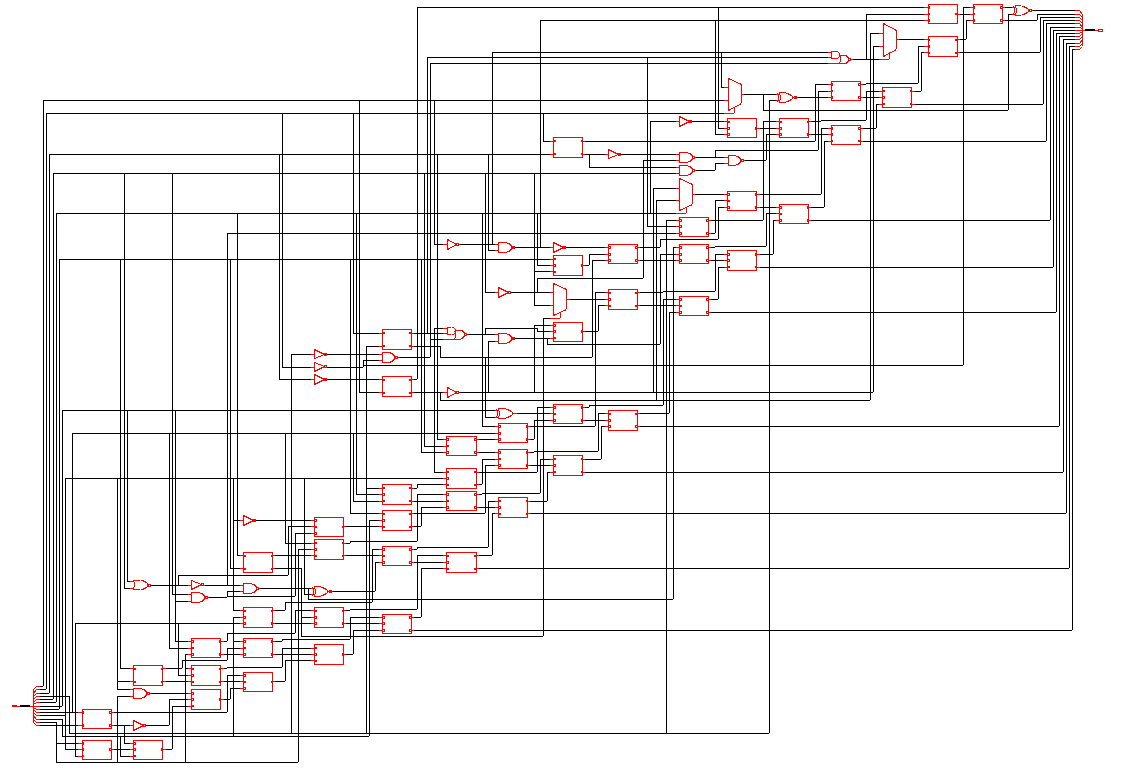
\includegraphics[width=1\textwidth]{img/13Bit_Konstantenmultiplizierer_neu.png}
  %}
  \caption{Schaltnetz des 13 Bit Konstantenmultiplizierers für $\frac{\sqrt{2}}{2} = 0.70711 \simeq 0.70703125 = 0001011010100_2$ in Encounter; Eingang links, Ausgang rechts.}
  \label{pic:Konstantenmultiplizierer}
\end{figure}

Der vollständige Gate-Report befindet sich in Abschnitt \ref{src:rc_gate_report_KonstMult} auf Seite \pageref{src:rc_gate_report_KonstMult}



\subsection{Bildung des 2er-Komplements eines 13 Bit Vektors}


In Abb. \ref{pic:13BitInverter} ist die nicht expliziet implementierte, aber in Abschnitt \ref{sec:RelleEingangswerte} erwähnte Negierung von Zahlen zu sehen.

\begin{figure}[htpb]
\centering
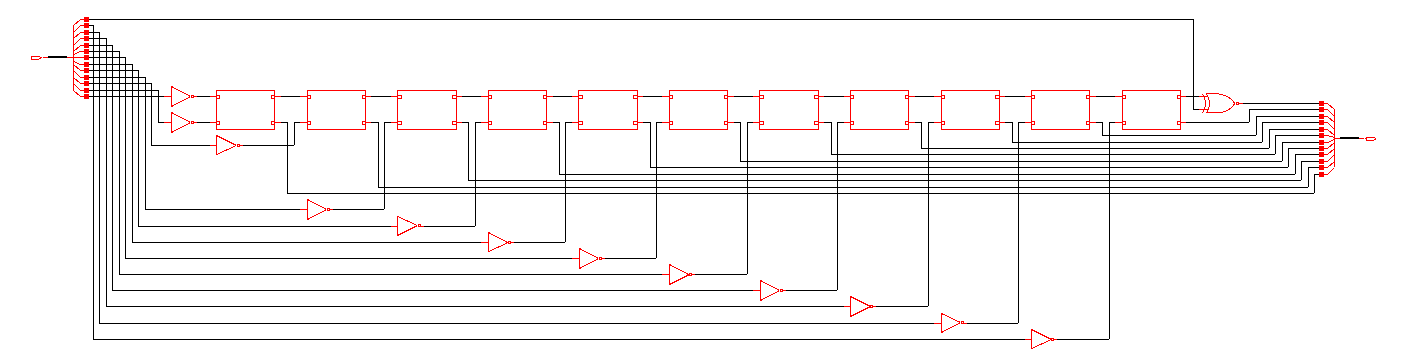
\includegraphics[width=0.99\textwidth]{img/13Bit_Negierer.png}
\caption{Schaltnetz einer Einheit zur Bildung des 2er-Komplements eines 13 Bit Vektors; Eingang links, Ausgang rechts.}
\label{pic:13BitInverter}
\end{figure}

Für die Negierung eines 13 Bit Vektors hat das Synthesewerkzeug \texttt{encounter} 22 Standardzellen verwendet. Das sind knapp doppelt so viele Gatter, wie der Vektor 
Bits breit ist. Der Unterschied zum Konstantenmultiplizierer fällt somit sehr gering aus. 
Wie zu sehen, handelt es sich fast ausschließlich um Inverter und Addierer. In Abschnitt \ref{sec:Integer2erKomplement} wurde bereits beschrieben, dass für die Bildung des
2er-Komplements zunächst alle Bits invertiert werden müssen. Abschließend wird auf den Vektor 1 LSB addiert. 
Beide Pfade weisen die gleiche Länge auf und verwenden überwiedend die selben
Gattertypen, weshalb darauf geschlossen werden kann, dass die maximale Gatterlaufzeit in der gleichen Größenordnung liegen muss.

\subsection{13 Bit Addierer}
Der 13 Bit Addierer hat zwei 13 Bit Eingänge, allerdings werden durch einen Bitshift beide Eingangswerte halbiert, damit kein Überlauf entsteht. Insofern fließen nur jeweils 
die forderen 12 Bit in die Berechnung ein.
\begin{figure}[htbp]
 \centering
 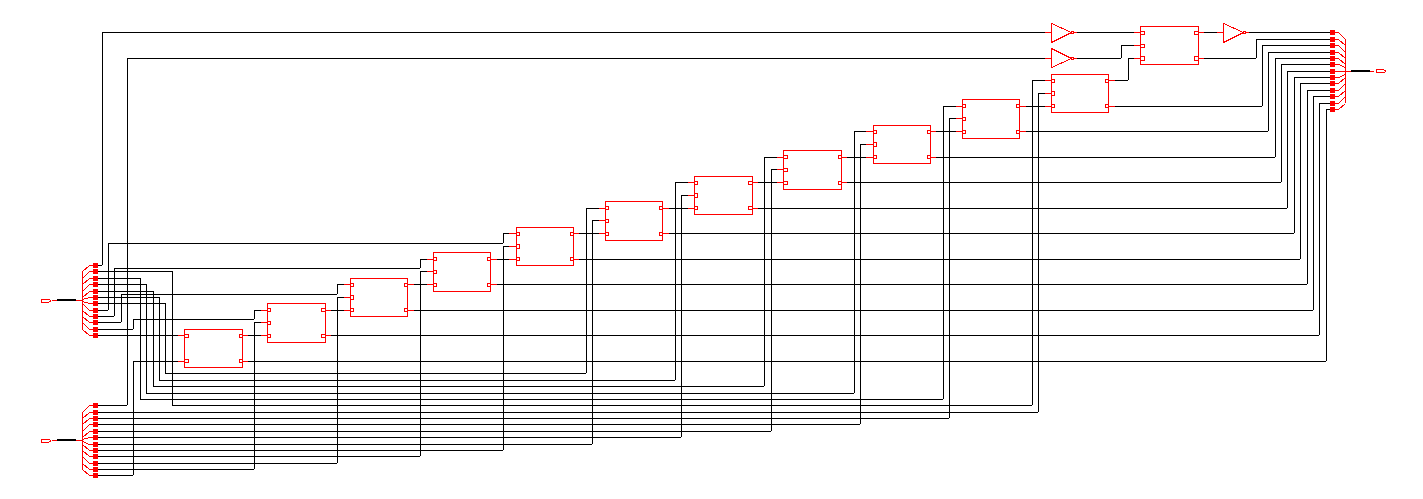
\includegraphics[width=0.99\textwidth]{img/13Bit_Addierer.png}
 \caption{Schaltnetz eines 12 Bit Addierers, Eingänge links (12\,Bit), Ausgang rechts (13\,Bit).}
 \label{pic:13BitAddierer}
\end{figure}

\subsection{Vergleich der Syntheseergebnisse}
 In Tabelle \ref{tab:VergleichSyntheseergebnisse} ist eine Gegenüberstellung der Syntheseergebnisse unter den Aspekten Anzahl der Gatter und Fläche.
\begin{table}[!ht]
\centering
 \caption{Vergleich der Syntheseergebnisse der Teilkomponenten in Bezug auf Anzahl der Gatter und ihre Fläche}
 \label{tab:VergleichSyntheseergebnisse}
 \begin{tabular}{lcc}
 \hline
				&Gatter  	&Fläche (Prozess: 350nm) \\
  \hline	
  13\,Bit Konstantenmultiplizierer für $\nicefrac{\sqrt{2}}{2}$	& 82		& $\SI{6612}{\um^2}$ \\
  13\,Bit regulärer Multiplizierer				& 194		& $\SI{21985}{\um^2}$\\
  12\,Bit Addierer						& 15		& $\SI{3257}{\um^2}$\\
  13\,Bit 2er-Komplement-Bildung				& 24		& $\SI{2147}{\um^2}$\\
  \hline
 \end{tabular}
\end{table}



\subsection{Gegenüberstellung der Konstantenmultiplikation und der Bildung des 2er-Komplements}

Unter diesem Punkt sollen die Konstantenmultiplikation und die Bildung des 2er-Komplements unter Aspekten der benötigten Zeit und des benötigten Platzes auf einem Chip 
betrachtet werden. Um einen Eindruck hiervon zu erhalten, werden im Kapitel Entwurf in Abschnitt \ref{sec:Syntheseergebnisse} jeweils die Schaltnetzte 
%für die Negation mittels 2er-Komplement und die Multiplikation mit einem konstanten Faktor 
gezeigt.
Wie dort erläutert, lässt sich anhand dieser sagen, dass es bei dieser Art der Implementierung keinen zeitlichen Gewinn gibt, da beide kritischen Pfade etwa gleich lang 
sind. Für die knapp $4$ mal mehr Gatter bei der Multiplikation ist auch ein größerer Vertrahtungsaufwandt erforderlich, sodass die Konstantenmultiplizierer
auf einem Chip eine etwas größere Fläche beanspruchen. Da es sich hier insgesamt aber um wenige Gatter handelt, wirkt sich dies erst bei sehr vielen Instanzen aus.
Es kann an dieser Stelle deshalb festgehalten werden, dass dieser Unterschied nicht als entscheidend geltend gemacht werden kann.



